\documentclass[10pt,twocolumn,letterpaper]{article}

    \usepackage{cvpr}
    \usepackage{times}
    \usepackage{epsfig}
    \usepackage{graphicx}
    \usepackage{amsmath}
    \usepackage{amssymb}
    
    % Include other packages here, before hyperref.
    
    % If you comment hyperref and then uncomment it, you should delete
    % egpaper.aux before re-running latex.  (Or just hit 'q' on the first latex
    % run, let it finish, and you should be clear).
    \usepackage[pagebackref=true,breaklinks=true,letterpaper=true,colorlinks,bookmarks=false]{hyperref}
    
    \cvprfinalcopy % *** Uncomment this line for the final submission
    
    \def\cvprPaperID{****} % *** Enter the CVPR Paper ID here
    \def\httilde{\mbox{\tt\raisebox{-.5ex}{\symbol{126}}}}
    
    % Pages are numbered in submission mode, and unnumbered in camera-ready
    \ifcvprfinal\pagestyle{empty}\fi
    \begin{document}
    
    %%%%%%%%% TITLE
    \title{Technical Report for First Project in Parallel Computing}
    
    \author{Yasheng Sun\\
    117020910076\\
    {\tt\small sunyasheng123@gmail.com}
    % For a paper whose authors are all at the same institution,
    % omit the following lines up until the closing ``}''.
    % Additional authors and addresses can be added with ``\and'',
    % just like the second author.
    % To save space, use either the email address or home page, not both
    }
    
    \maketitle
    %\thispagestyle{empty}
    
    %%%%%%%%% ABSTRACT
    \begin{abstract}
       This report concludes the first project in parallel computing. 
       This project involves the basic usage of MPI function and 
       application of MPI in Mento Carto Method, which is illustrated through 
       approximation of $\pi$. 
       All my code is publicly available on my github 
       \url{https://github.com/sunyasheng/Parallel-Computing}.

    \end{abstract}
    
    %%%%%%%%% BODY TEXT
    \section{Hello World}
    This problem involves basic usage of MPI function as is shown in Table~\ref{command_table}.  
    \begin{table}
        \begin{center}
        \begin{tabular}{|c|c|}
        \hline
        function & meaning\\
        \hline
        MPI\_Comm\_size & get number of processors \\
        MPI\_Comm\_rank & get id of current processor \\
        MPI\_Get\_processor\_name & get name of current processor \\
        MPI\_Wtime & get the current time\\
        \hline
        \end{tabular}
        \end{center}
        \caption{Basic function of MPI.}
        \label{command_table}
    \end{table}
    \subsection{Result}
    The output of this first hello world MPI program is presented in Fig.~\ref{hello_world}.
    It is just some navie ouputs which notify us that there are actually multiple threads 
    runing this program.
    \begin{figure}[t]
        \begin{center}
           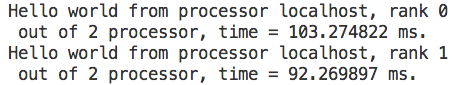
\includegraphics[width=1.\linewidth]{images/hello_world.png}
        \end{center}
           \caption{Ouput in the Hello World project.}
        \label{fig:long}
        \label{fig:onecol}
        \label{hello_world}
    \end{figure}
    
    \section{Computation of $\pi$ through Mento Carto Method}
    This project involves a MPI program to approximate the $\pi$. Mento Carto method is a 
    common simulation method to do approximation in computation. In this section, we will
    first introduce the method to finish the $\pi$ approximation problem and then illustrated
    the result.
    \subsection{Methodology}
    
    Here we use the Mento Corto method to compute $\pi$. The basic principle to 
    compute $\pi$ is shown in Fig.~\ref{mentoCarlo}. We sample the points randomly in 
    the green square, whose locations are split into two subsets. $\pi$ is approximated 
    by calculating the fraction of all the points located inside the circle. 
    \begin{figure}[t]
        \begin{center}
           
\includegraphics[width=0.8\linewidth]{images/computation.png}
        \end{center}
           \caption{Illustration of $\pi$ computation through Mento Carlo Method. $\pi$ is
           approximated by the fraction of points located in the circle.}
        \label{fig:long}
        \label{fig:onecol}
        \label{mentoCarlo}
    \end{figure}
    
    In this project, we just achieve the parallel vision of the above approach. Mutiple threads are launched and each of them 
    holds a bunch of particles which will locate inside the square randomly. For each thread, we count the 
    number of particles belong to the circle. After that, we sum up all these numbers in different processors
    and divide it by the total number of particles to obtain  $\pi$ in the reduced processor. 
    
    \subsection{Result}
    \begin{table}
        \begin{center}
        \begin{tabular}{|c|c|c|}
        \hline
        processor number  &  estimated value & consumed time \\
        \hline
        1 &  3.126 & 69.95ms\\
        2 & 3.138 &  90.72ms\\
        \hline
        \end{tabular}
        \end{center}
        \caption{Estimated value and consumed time with different number of particles.}
        \label{process_number}
    \end{table}
    \begin{table}
        \begin{center}
        \begin{tabular}{|c|c|c|}
        \hline
        load particles number  &  estimated value & consumed time \\
        \hline
        10000 &  3.134 & 98.14ms\\
        100000 & 3.142 & 142.95ms\\
        \hline
        \end{tabular}
        \end{center}
        \caption{Estimated value and consumed time under different load number of particles in 
        each processors.}
        \label{load_number}
    \end{table}
    
    The estimated value and consumed time under different number of processors when the load number of particles 
    is 10000 is given in Table~\ref{process_number}. The estimated value and consumed time
    under different load number of particles when the processor number is 2 is given in Table~\ref{load_number}.
    With the increasing number of the processors or increasing number of particles in every processors
    , the estimated number approximates true value more accurately since total number of particles here equals
    their mutiplication. More involved particles lead to a more precise result. In the meantime, longer
    time is required because time consumption in each processor is increased and the reduced processor has to wait all other processors finish before 
    reduction. 
    \section{Conclusion}
    In this project, we explore the basic usage of MPI function through a $\pi$ estimation
    task. Experiment shows that the approximation accuracy can be improved by adding more 
    particles with cost of time consumption. Future work will involve more complicated 
     task under more advanced parallel framework.

    
    {\small
    \bibliographystyle{ieee}
    \bibliography{egbib}
    }
    \begin{thebibliography}{1}

    \bibitem{IEEEhowto:kopka}
    % H.~Kopka and P.~W. Daly, \emph{A Guide to \LaTeX}, 3rd~ed.\hskip 1em plus
    % 0.5em minus 0.4em\relax Harlow, England: Addison-Wesley, 1999.
    % D. Pathak, R. Girshick, P. Doll ́ ar, T. Darrell, and B. Hariha-ran.
    % Learning features by watching objects move. In \emph{CVPR}, 2017.
    https://www.openmp.org/wp-content/uploads/Intro\_To\_OpenMP\_Mattson.pdf
    \end{thebibliography}

    \end{document}